\chapter{Teoria}
\label{cap:teoria}

\section{Conjunts}

Partint de la noció intuïtiva de conjunt, en aquesta secció
desenvoluparem les propietats bàsiques dels conjunts. L'objectiu
d'aquesta breu exposició serà aconseguir que et familiaritzis amb la
terminologia i les notacions que s'introdueixen i que s'empraran en totes
les altres unitats didàctiques. És recomanable, abans de continuar, fer
una lectura comprensiva dels apunts «Lògica, raonament
i demostració».

\subsection{Les nocions d'element, conjunt i pertinença}

Una caixa de boles, un raïm o un àlbum de fotos són tots
exemples de conjunts de coses o col·leccions d'objectes.
La noció de conjunt és fonamental en totes les branques de les matemàtiques. Per exemple:

\begin{itemize}
\item En geometria plana es diu circumferència el conjunt de punts que són equidistants d'un punt fix donat.

\item En àlgebra es parla del conjunt dels nombres parells que està
format per tots els enters que són divisibles per 2.

\item En càlcul s'anomena domini d'una funció real de variable real
el conjunt de nombres reals pels quals hi ha ben definida la seva imatge.
\end{itemize}

Emprarem la paraula \textbf{conjunt} com a sinònim de
col·lecció d'objectes. Els objectes que formen un
conjunt es diuen \textbf{elements} del conjunt. D'aquesta manera, direm que
un conjunt està format per elements o que uns determinats elements
formen un conjunt.

\bigskip

Ara bé, un conjunt estarà ben definit si és possible donar un
criteri que permeti decidir si un element donat qualsevol pertany o no al
conjunt. Per exemple, les boles vermelles d'aquesta caixa o les fotos d'en
Miquel en aquest àlbum són conjunts ben definits. En el primer cas,
una bola de la caixa és del conjunt si és vermella i, en el segon,
una foto és del conjunt si hi apareix en Miquel. Observa, però, que,
en ambdós casos, abans de definir els conjunts anteriors tenim els
elements: les boles de la caixa i les fotos de l'àlbum.

\bigskip

Si ara simbolitzem per $U$ una determinada col·lecció
d'objectes, llavors diem que uns determinats objectes d'$U$ formen un
conjunt $A$ i si $x$ simbolitza un element d'$A$, aleshores direm que
l'element $x$ \textbf{pertany} al conjunt $A$ i escriurem%
\begin{equation*}
x\in A\text{.}
\end{equation*}
Si $x$ és un element d'$U$, però no és un element de $A$, direm
que l'element $x$ no pertany al conjunt $A$ i escriurem%
\begin{equation*}
x\notin A\text{.}
\end{equation*}
El símbol matemàtic $\in$ s'interpreta com la relació de
pertinença que s'estableix entre elements i conjunts. Per consegüent, un conjunt està determinat per una relació de pertinença a
ell. Tot i això, com veurem més endavant (quan parlem del conjunt de
parts d'un conjunt donat), un element pot ser alhora un conjunt i un conjunt
pot ser un element d'un altre conjunt.

\bigskip

Per cursos anteriors, tenim coneixement de l'existència d'alguns
conjunts numèrics l'ús dels quals és molt freqüent en les
matemàtiques i que es designen amb símbols especials. Així,
tenim

\begin{equation*}
\begin{tabular}{c|c}
Conjunts numèrics & Símbol \\ \hline
Naturals & $\mathbb{N}$ \\
Enters & $\mathbb{Z}$ \\
Racionals & $\mathbb{Q}$ \\
Reals & $\mathbb{R}$ \\
Complexos & $\mathbb{C}$%
\end{tabular}
\ \
\end{equation*}

\begin{exemple}
Pel coneixement que d'ells ja tenim, podem escriure les següents
relacions:%
\begin{equation*}
\begin{tabular}{lllllll}
$-2\notin\mathbb{N}$ &  & $-3\in\mathbb{Z}$ &  & $\sqrt{2}\notin\mathbb{Q}$
&  & $\sqrt[3]{5}\in\mathbb{R}$ \\
&  &  &  &  &  &  \\
$1\in\mathbb{N}$ &  & $\dfrac{1}{2}\notin\mathbb{Z}$ &  & $2.3555...\in
\mathbb{Q}$ &  & $1+i\notin\mathbb{R}$%
\end{tabular}
\
\end{equation*}
\end{exemple}

\subsection{Formes de definir conjunts}

Direm que un conjunt està determinat per \textbf{extensió} si donem
una llista de tots els seus elements. En aquest cas, escriurem els elements
entre claus separats per comes. Per exemple, el conjunt $A$ format pels nombres
\begin{equation*}
1,2,3
\end{equation*}
l'escriurem per%
\begin{equation*}
A=\{1,2,3\}\text{.}
\end{equation*}

\bigskip

Un conjunt està determinat per \textbf{comprensió} si donem una
condició que satisfan tots els seus elements. Així, el conjunt
anterior el podem definir per comprensió dient que $A$ és el conjunt
format pels nombres enters positius menors que quatre. En aquest últim
cas escriurem%
\begin{equation*}
A=\{x\in\mathbb{Z}:0<x<4\}
\end{equation*}
i es llegeix com «$A$ és el conjunt de nombres enters
que són més grans que 0 i menors que $4$». En general, si $%
P(x)$ expressa una condició o propietat que depèn d'una variable $x$%
, llavors%
\begin{equation*}
B=\left\{ x\in U:P(x)\right\}
\end{equation*}
designa el conjunt dels elements d'$U$ que satisfan la propietat $P(x)$.

\bigskip

Pot passar que no hi hagi cap element del conjunt de referència que
satisfaci una determinada propietat. Per aquesta raó, admetem l'existència
d'un conjunt que no conté elements, que anomenem \textbf{conjunt buit}
i que designem amb el símbol $\emptyset$. D'aquesta manera,
per a tot $x$ la relació%
\begin{equation*}
x\in\emptyset
\end{equation*}
és sempre falsa, i%
\begin{equation*}
x\notin\emptyset
\end{equation*}
és sempre vertadera.

\bigskip

És instructiu representar gràficament un conjunt mitjançant una
regió tancada del pla de manera que tots els elements del conjunt
estiguin tancats en aquesta regió. Es diuen \textbf{diagrames de Venn} i
es construeixen com s'indica en el següent gràfic, on hem
representat el conjunt $A=\{a,b,e\}$.\par\smallskip
\begin{center}
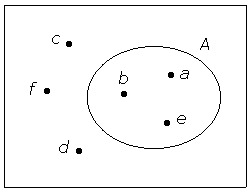
\includegraphics[width=6.7107cm]{img/set1.jpg}
\end{center}
\smallskip\par

\begin{observacio}
Observa que no hem definit els conceptes de conjunt i element. En el seu
lloc, hem intentat donar una idea intuïtiva clara de totes dues
nocions. En cursos més avançats es pot veure que en la construcció axiomàtica d'una teoria de conjunts, els termes «conjunt» i «pertinença» no es defineixen i s'empren sense explicar el seu
significat. Un conjunt serà qualsevol cosa que satisfaci els axiomes de
la teoria. D'aquesta manera, no hi ha dubte que la intuïció sobre
la qual es basa la teva noció de conjunt pot estar equivocada, però
del que es tracta no és tant saber què són els conjunts, sinó què podem fer amb ells correctament. Això últim és el que
volem fer aquí.
\end{observacio}

\begin{observacio}
Podria semblar natural admetre que tota condició $P(x)$ defineix un
conjunt%
\begin{equation}
\{x:x\text{ compleix }P(x)\}\text{,}   \label{3}
\end{equation}
però, d'aquesta manera, resulta que hi ha condicions «rares» que donen lloc a «conjunts» contradictoris sobre els quals no és
possible raonar. Per exemple, si considerem la condició $x\notin x$
(tots els conjunts que no són elements de si mateixos) i denotem per $B$
el «conjunt» d'elements que satisfan
aquesta condició, és a dir,%
\begin{equation*}
B=\{x:x\notin x\}
\end{equation*}
llavors es compleix%
\begin{equation*}
\left( \forall x\right) (x\in B\Longleftrightarrow x\notin x)
\end{equation*}
i, en particular, també es compleix%
\begin{equation*}
B\in B\Longleftrightarrow B\notin B
\end{equation*}
cosa que, evidentment, constitueix una contradicció. Per a evitar aquests
absurds, és preferible limitar la condició als elements d'algun
conjunt ja conegut $U$. Per aquest motiu hem escrit%
\begin{equation*}
\{x\in U:x\text{ compleix }P(x)\text{\}}
\end{equation*}
en lloc de (\ref{3}).
\end{observacio}

\subsection{Igualtat i inclusió entre conjunts}

Direm que dos conjunts $A$ i $B$ són \textbf{iguals} si contenen els
mateixos elements, és a dir, si per a cada $x$, $x\in A$ equival a $x\in
B$. En símbols
\begin{equation*}
\left( \forall x\right) \left( x\in A\Longleftrightarrow x\in B\right)
\end{equation*}
i es llegeix «per a tot $x$, $x$ és de $A$ si i només si $x$ és de $B$». Si els conjunts $A$ i $B$ són
iguals, escriurem%
\begin{equation*}
A=B
\end{equation*}
i la seva negació per a%
\begin{equation*}
A\neq B\text{.}
\end{equation*}

El símbol matemàtic $=$ s'interpreta com la relació d'igualtat
que s'estableix entre conjunts. A partir de la definició, és
immediat comprovar que aquesta relació satisfà les següents
propietats:

\begin{enumerate}
\item Per a tot conjunt $A$, $A=A$.

\begin{prova}
Sabem que $x\in A\Longleftrightarrow x\in A$ és una equivalència lògica. Com $x$ és un element arbitrari d'$A$, aleshores es compleix $%
\left( \forall x\right) \left( x\in A\Longleftrightarrow x\in A\right) $ i,
com a consequència, $A=A$.
\end{prova}

\item Donats dos conjunts $A$ i $B$, si $A=B$ llavors $B=A$.

\begin{prova}
Sabem que per a tot $x$, es té que $x\in A\longleftrightarrow x\in B$
és equivalent a $x\in B\longleftrightarrow x\in A$ i, per tant, si $A=B$%
, llavors $B=A$.
\end{prova}

\item Donats tres conjunts $A$, $B$ i $C$, si $A=B$ i $B=C$, llavors $A=C$.

\begin{prova}
Sabem que per a tot $x$, es té que $x\in A\longleftrightarrow x\in B$ i $
x\in B\longleftrightarrow x\in C$. Llavors, per la propietat transitiva del
bicondicional es té $x\in A\longleftrightarrow x\in C$ i, per tant, si $%
A=B$ i $B=C$, llavors $A=C$.
\end{prova}
\end{enumerate}

\bigskip

Si $A$ i $B$ són dos conjunts tals que tot element d'$A$ és també
un element de $B$, és a dir,
\begin{equation*}
\left( \forall x\right) \left( x\in A\Longrightarrow x\in B\right) \text{,}
\end{equation*}
llavors es diu que $A$ és un \textbf{subconjunt} de $B$ o que $A$ està \textbf{inclòs} en $B$ i se simbolitza per a%
\begin{equation*}
A\subset B\text{ \ \ \ \ o \ \ \ }B\supset A\text{.}
\end{equation*}

Mitjançant diagrames de Venn, representem aquest fet així\par\smallskip
\begin{center}
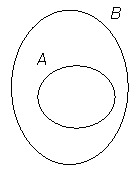
\includegraphics[width=3.7474cm]{img/set2.jpg}\\
{\small $A\subset B$}
\end{center}
\smallskip\par

Si $A\subset B$ i $A\neq B$ es diu que $A$ és un \textbf{subconjunt propi%
} de $B$. El símbol matemàtic $\subset$ s'interpreta com la relació d'inclusió que s'estableix entre conjunts; en particular,
simbolitzem per $A\varsubsetneq B$ el fet que $A$ és un subconjunt propi
de $B$. A partir de la definició i regles de deducció lògica,
és immediat comprovar que aquesta relació satisfà les següents propietats:

\begin{enumerate}
\item Per a tot conjunt $A$, $A\subset A\,$.

\item Donats dos conjunts $A$ i $B$, si $A\subset B$ i $A\supset B$, llavors
$A=B$.

\item Donats tres conjunts $A$, $B$ i $C$, si $A\subset B$ i $B\subset C$,
llavors $A\subset C$.
\end{enumerate}

\bigskip

\begin{exemple}
Observa que es compleixen les següents relacions:

\begin{itemize}
\item $\emptyset\subset A$

\item $\left\{ 1\right\} \subset\left\{ 1,2,3\right\} $

\item $\{2,4\}\subset\left\{ x\in\mathbb{N}:x\text{ és parell}\right\} $

\item $\{x\in\mathbb{Z}:0<x<4\}\varsubsetneq\left\{ x\in\mathbb{Z}%
:x^{2}-3x+2=0\right\} $
\end{itemize}
\end{exemple}

\subsection{Operacions amb conjunts}

En aquest apartat veurem com podem construir nous conjunts a partir d'uns
altres ja donats. Suposem que existeix un conjunt $U$ que anomenem \textbf{%
univers} i del qual prendrem tots els subconjunts.

\subsubsection{Parts d'un conjunt}

Si $A$ és un conjunt, es diu \textbf{conjunt de parts} d'$A$ el conjunt
els elements del qual són tots els subconjunts d'$A$ i es designa per $%
\mathcal{P}(A)$. Així, tenim%
\begin{equation*}
\mathcal{P}(A)=\left\{ x\subset U:x\subset A\right\} \text{.}
\end{equation*}
Observa que $\mathcal{P}(A)$ és un conjunt els elements del qual són
alhora conjunts.

\bigskip

\begin{exemple}
Observa que si $A=\{a,b,c\}$, llavors%
\begin{equation*}
\mathcal{P}(A)=\{\emptyset ,\{a\},\{b\},\{c\},\{a,b\},\{a,c\},\{b,c\},A\}%
\text{.}
\end{equation*}
\end{exemple}

\subsubsection{Unió de dos conjunts}

Si $A$ i $B$ són conjunts, es diu \textbf{unió} d'$A$ i $B$ al
conjunt simbolitzat per $A\cup B$ que té per elements tots els que
pertanyen a $A$ o a $B$ o als dos alhora. Mitjançant diagrames de Venn,
representem aquest fet així \par\smallskip
\begin{center}
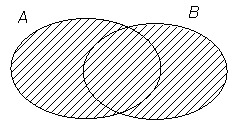
\includegraphics[width=2.4863in]{img/set3.jpg}\\
{\small $A\cup B$}
\end{center}
\smallskip\par
Simbòlicament, escrivim%
\begin{equation*}
A\cup B=\{x\in U:x\in A\text{ ~o~ }x\in B\}
\end{equation*}

\begin{exemple}
Observa que si $A=\left\{ 1,2,3\right\} $ i $B=\left\{ 3,4,5\right\} $,
llavors%
\begin{equation*}
A\cup B=\left\{ 1,2,3,4,5\right\} \text{.}
\end{equation*}
\end{exemple}

\subsubsection{Intersecció de dos conjunts}

Si $A$ i $B$ són conjunts, es diu \textbf{intersecció} d'$A$ i $B$
al conjunt denotat per $A\cap B$ que té per elements tots els que
pertanyen tant a $A$ com a $B$. El diagrama de Venn que representa aquest
fet és el següent: \par\smallskip
\begin{center}
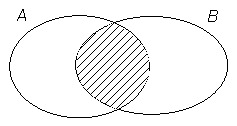
\includegraphics[width=6.3417cm]{img/set4.jpg}\\
{\small $A\cap B$}
\end{center}
\smallskip\par Simbòlicament, escrivim%
\begin{equation*}
A\cap B=\{x\in U:x\in A\text{ ~i~ }x\in B\}
\end{equation*}

Si $A\cap B=\emptyset$, llavors es diu que els conjunts $A$ i $B$ són
\textbf{disjunts}, o sigui que no tenen res en comú.

\begin{exemple}
Observa que si $A=\left\{ 1,2,3\right\} $ i $B=\left\{ 3,4,5\right\} $,
llavors%
\begin{equation*}
A\cap B=\left\{ 3\right\} \text{.}
\end{equation*}
\end{exemple}

\subsubsection{Propietats de la unió i de la intersecció de conjunts}

Donats tres conjunts qualssevol $A$, $B$ i $C$ es compleixen les següents relacions:

\begin{enumerate}
\item $A\cup A=A$ i $A\cap A=A$

\item $A\cup(B\cup C)=(A\cup B)\cup C$ i $A\cap(B\cap C)=(A\cap B)\cap C$

\item $A\cup B=B\cup A$ i $A\cap B=B\cap A$

\item $A\cup(B\cap C)=(A\cup B)\cap(A\cup B)$ i $A\cap(B\cup C)=(A\cap
B)\cup(A\cap C)$

\item $A\cup(B\cap A)=A$ i $A\cap(B\cup A)=A$

\item $A\cup\emptyset=A$ i $A\cap\emptyset=\emptyset$
\end{enumerate}

Les demostracions d'aquestes propietats les trobaràs en els exercicis
resolts.

\subsubsection{Diferència entre dos conjunts}

Si $A$ i $B$ són conjunts, es diu \textbf{diferència} entre $A$ i $B$
al conjunt denotat per $A\setminus B$ i que té per elements tots els que
pertanyen a $A$ i que no són de $B$. El diagrama de Venn en aquest cas
és:\par\smallskip
\begin{center}
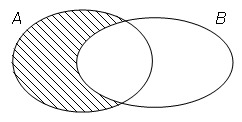
\includegraphics[width=2.5486in]{img/set5.jpg}\\
{\small $A-B$}
\end{center}
\smallskip\par Simbòlicament,
escrivim%
\begin{equation*}
A-B=\{x\in U:x\in A\text{ ~i~ }x\notin B\}
\end{equation*}

\begin{exemple}
Si $A=\left\{ 1,2,3\right\} $ i $B=\left\{ 3,4,5\right\} $, llavors es té%
\begin{equation*}
A-B=\left\{ 1,2\right\} \text{.}
\end{equation*}
\end{exemple}

\subsubsection{Complementari d'un conjunt}

Donat un conjunt $A$, es diu \textbf{complementari} d'$A$ al conjunt denotat
per $\complement A$ i que té per elements tots els que són de
l'univers $E$ i no pertanyen a $A$.\par\smallskip
\begin{center}
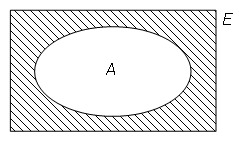
\includegraphics[width=2.5175in]{img/set6.jpg}\\
{\small $\complement A$}
\end{center}
\smallskip\par
En altres paraules, es té%
\begin{equation*}
\complement A=\{x\in E:x\notin A\}\text{.}
\end{equation*}
És evident que es compleix%
\begin{equation*}
\complement A=E-A\text{.}
\end{equation*}

\begin{exemple}
Si $E=\mathbb{R}$ i $A=\left\{ x\in\mathbb{R}:\left\vert x\right\vert
=1\right\} $, llavors es té%
\begin{equation*}
\complement_{E}A=\mathbb{R}-\left\{ -1,1\right\}
\end{equation*}
\end{exemple}

\subsubsection{Propietats del complementari d'un conjunt}

Si $U$ és l'univers, llavors es compleixen les següents propietats:

\begin{enumerate}
\item $\complement U=\emptyset$ i $\complement\emptyset=U$

\item $\complement\left( \complement A\right) =A$

\item Lleis de De Morgan: $\complement\left( A\cup B\right) =\complement
A\cap\complement B$ i $\complement\left( A\cap B\right) =\complement
A\cup\complement B$
\end{enumerate}

Les demostracions d'aquestes propietats les trobaràs en els exercicis
resolts.

\subsection{Parell ordenat i producte cartesià de dos conjunts}

Es diu \textbf{parell ordenat} de dos elements $x$ i $y$ al conjunt denotat
per $(x,y)$ que té per elements els conjunts $\left\{ x\right\} $ i $
\left\{ x,y\right\} $, és a dir,%
\begin{equation*}
(x,y)=\left\{ \left\{ x\right\} ,\left\{ x,y\right\} \right\} \text{.}
\end{equation*}
Llavors, diem que $x$ és la \textbf{primera component} i $y$ és la
\textbf{segona component} del parell ordenat $(x,y)$. Per la definició
d'igualtat de conjunts, és fàcil deduir que es compleix%
\begin{equation*}
\begin{array}{ccc}
\left\{ a,b\right\} =\left\{ c,d\right\} & \Longleftrightarrow & a=c\text{ i
}b=d\text{ o bé }a=d\text{ i }b=c%
\end{array}
\end{equation*}
mentre que%
\begin{equation*}
\begin{array}{ccc}
(a,b)=(c,d) & \Longleftrightarrow & a=c\text{ i }b=d%
\end{array}
\end{equation*}
Per tant, l'única diferència entre els conjunts $\left\{ x,y\right\}
$ i $(x,y)$ resideix en l'ordre. Si $x$ i$\ y$ són dos elements
diferents, llavors $\left\{ x,y\right\} =\left\{ y,x\right\} $ i, en canvi, $%
(x,y)\neq(y,x)$.

\bigskip

Donats dos conjunts $A$ i $B$, es diu \textbf{producte cartesià} d'$A$ i
$B$ al conjunt denotat per $A\times B$ que té per elements tots els
parells ordenats la primera component dels quals és un element d'$A$ i
la segona component és un element de $B$, simbòlicament escrivim
\begin{equation*}
A\times B=\left\{ (x,y):x\in A\text{ i }y\in B\right\} \text{.}
\end{equation*}

\begin{exemple}
Si $A=\left\{ 1,2\right\} $ i $B=\left\{ a,b\right\} $, llavors es té%
\begin{equation*}
A\times B=\left\{ (1,a),(1,b),(2,a),(2,b)\right\}
\end{equation*}
Observa que%
\begin{equation*}
B\times A=\left\{ (a,1),(a,2),(b,1),(b,2)\right\}
\end{equation*}
i és evident que $A\times B\neq B\times A$.
\end{exemple}

\section{Relacions}

Identifiquem les relacions amb conjunts de parells ordenats i, per tant, amb
subconjunts del producte cartesià de dos conjunts donats. Que un parell
ordenat pertanyi a una relació significa que la relació en qüestió es dona entre el primer component del parell i el segon.

\subsection{Relacions entre dos conjunts}

Donats dos conjunts $A$ i $B$, es diu \textbf{relació} entre $A$ i $B$ a
tot subconjunt de $A\times B$. Si $R\subset A\times B$ és una relació
entre $A$ i $B$, llavors quan es compleix que $(a,b)\in R$ diem que la relació \textbf{es dona} entre $a$ i $b$, o simplement, que $a$ \textbf{està relacionat amb} $b$.

\begin{exemple}
Si $A=\{1,2\}$ i $B=\{a,b\}$, llavors $R=\left\{ (1,a),(2,b)\right\} $, $%
S=\left\{ (1,a)\right\} $ i $T=\left\{ (2,a),(2,b)\right\} $ són
relacions entre $A$ i $B$ i, en canvi, $J=\left\{ (a,2),(2,1)\right\} $ no
ho és.
\end{exemple}

Per ser conjunts, si $R$ i $S$ són relacions entre $A$ i $B$, llavors 
$R=S$ si i només si $R$ i $S$ contenen els mateixos parells ordenats. Es
diu \textbf{domini} d'una relació $R$ entre $A$ i $B$ al conjunt denotat
per $\mathcal{D}\left( R\right) $ que té per elements les primeres
components dels parells ordenats de $R$. Es diu \textbf{recorregut} de $R$
el conjunt denotat per $\mathcal{R}\left( R\right) $ que té per elements
les segones components dels parells ordenats de $R$. Així, tenim%
\begin{equation*}
\mathcal{D}\left( R\right) =\left\{ x:x\in A\text{ i existeix }y\in B\text{
tal que }(x,y)\in R\right\}
\end{equation*}
i%
\begin{equation*}
\mathcal{R}\left( R\right) =\left\{ y:y\in B\text{ i existeix }x\in A\text{
tal que }(x,y)\in R\right\} \text{.}
\end{equation*}

\begin{exemple}
Si $A=\{1,2\}$, $B=\{a,b\}$ i $R=\left\{ (2,a),(2,b)\right\} $ és una
relació entre $A$ i $B$, llavors $\mathcal{D}\left( R\right) =\left\{
2\right\} $ i $\mathcal{R}\left( R\right) =\left\{ a,b\right\} =B$.
\end{exemple}

\subsection{Relacions binàries en un conjunt}

Si $A$ és un conjunt, diem que $R$ és una \textbf{relació binària} en $A$ si $R\subset A\times A$. En tot conjunt $A$ sempre podem
definir les relacions binàries següents:

\begin{enumerate}
\item Relació d'identitat en $A$: $I_{A}=\left\{ (x,x):x\in A\right\} $

\item Relació nul·la en $A$: $\emptyset$

\item Relació total en $A$: $A\times A$
\end{enumerate}

\bigskip

Considerem un conjunt $A$ i una relació binària $R\subset A\times A$%
. Distingim les següents propietats de $R$:

\begin{enumerate}
\item $R$ és \textbf{reflexiva}: per a tot $x\in A$, $(x,x)\in R$

\item $R$ és \textbf{irreflexiva}: per a tot $x\in A$, $(x,x)\notin R$

\item $R$ és \textbf{simètrica}: per a tot $x,y\in A$, si $(x,y)\in R
$ llavors $(y,x)\in R$

\item $R$ és \textbf{asimètrica}: per a tot $x,y\in A$, si $(x,y)\in
R$ llavors $(y,x)\notin R$

\item $R$ és \textbf{antisimètrica}: per a tot $x,y\in A$, si $%
(x,y)\in R $ i $(y,x)\in R$, llavors $x=y$

\item $R$ és \textbf{transitiva}: per a tot $x,y,z\in A$, si $(x,y)\in R$
i $(y,z)\in R$, llavors $(x,z)\in R$
\end{enumerate}

\begin{exemple}
Si $A=\left\{ 1,2,3\right\} $ i $R=\left\{ (1,2),(2,3),(2,2),(1,3)\right\} $%
, llavors es compleix:

\begin{itemize}
\item $R$ no és reflexiva, doncs $(1,1)\notin R$.

\item $R$ no és irreflexiva, doncs $(2,2)\in R$.

\item $R$ no és simètrica, perquè $(1,2)\in R$ i $(2,1)\notin R$.

\item $R$ no és asimètrica, doncs $(2,2)\in R$.

\item $R$ és antisimètrica, perquè no hi ha cap parell
d'elements diferents $x,y$ tals que $(x,y)\in R$ i $(y,x)\in R$.

\item $R$ és transitiva, perquè no hi ha tres elements $x,y,z$ tals
que $(x,y)\in R$ i $(y,z)\in R$ i $(x,z)\notin R$.
\end{itemize}
\end{exemple}

\subsection{Relacions d'equivalència}

Donat un conjunt $A$ i una relació binària $R$ en $A$, diem que $R$
és una \textbf{relació d'equivalència} si $R$ és reflexiva,
simètrica i transitiva.

Tota relació d'equivalència $R$ en un conjunt $A$ ens permet
classificar els elements del conjunt en classes d'equivalència. Es diu
\textbf{classe d'equivalència} d'un element $a\in A$ al conjunt denotat
per $\left[ a\right] $ que té per elements tots els elements d'$A$ que
estan relacionats amb $a$. Així, tenim%
\begin{equation*}
\left[ a\right] =\left\{ x\in A:(x,a)\in R\right\} \text{.}
\end{equation*}

De la definició de classe d'equivalència, deduïm de seguida que%
\begin{equation*}
\begin{array}{ccc}
\left[ a\right] =\left[ b\right] & \Longleftrightarrow & (a,b)\in R%
\end{array}
\end{equation*}
o bé,%
\begin{equation*}
\begin{array}{ccc}
\left[ a\right] =\left[ b\right] & \Longleftrightarrow & \left( a\in\left[ b%
\right] \Longleftrightarrow b\in\left[ a\right] \right)%
\end{array}
\end{equation*}

Llavors es diu \textbf{conjunt quocient} de $A$ per la relació $R$ al
conjunt denotat per $A/R$ que té per elements les classes d'equivalència de tots els elements d'$A$ respecte de $R$. Així, tenim%
\begin{equation*}
A/R=\left\{ \left[ a\right] :a\in A\right\}
\end{equation*}

Quan $R$ és d'equivalència diem que el conjunt quocient $A/R$ és
una \textbf{partició} del conjunt $A$, això vol dir que és una
col·lecció de subconjunts no buits d'$A$, disjunts
dos a dos, i tals que la seva unió és $A$. Podem expressar això
afirmant que en $A/R$ es compleixen les següents propietats:

\begin{enumerate}
\item Per a tot $a\in A$, $\left[ a\right] \neq\emptyset$.

\item Per a tot $a,b\in A$ i $\left[ a\right] \neq\left[ b\right] $, $\left[
a\right] \cap\left[ b\right] =\emptyset$.

\item $\dbigcup A/R=A$, on $\dbigcup A/R$ és la unió de totes les
classes d'equivalència, doncs $A/R$ és el conjunt els elements del
qual són els que pertanyen a alguna classe de $A/R$, o sigui
\begin{equation*}
\begin{array}{ccc}
x\in\dbigcup A/R & \Longleftrightarrow & \text{existeix alguna classe }\left[
a\right] \in A/R\text{ tal que }x\in\left[ a\right] \text{.}
\end{array}
\end{equation*}
\end{enumerate}

És habitual usar $\sim$ o $\equiv$ com a símbols de relacions
d'equivalència sobre un conjunt.

\begin{exemple}
En el conjunt dels nombres enters $\mathbb{Z}$ es defineix la següent
relació binària $\equiv$%
\begin{equation*}
\begin{array}{ccc}
x\equiv y & \Longleftrightarrow & x-y\text{ és múltiple de }3%
\end{array}
\end{equation*}
És immediat comprovar que $\equiv$ és una relació d'equivalència en $\mathbb{Z}$:

\begin{itemize}
\item $\equiv$ és reflexiva: per a tot $x\in\mathbb{Z}$, $x\equiv x$
doncs $x-x=0$, que és un múltiple de $3$.

\item $\equiv$ és simètrica: per a tot $x,y\in\mathbb{Z}$, si $%
x\equiv y$, és a dir si $x-y$ és un múltiple de $3$, llavors 
$-(x-y)=y-x$ també és un múltiple de $3$ i, per tant, $y\equiv x$.

\item $\equiv$ és transitiva: per a tot $x,y,z\in\mathbb{Z}$, si $%
x\equiv y$ i $y\equiv z$, és a dir, si $x-y$ i $y-z$ són múltiples de $3$, també ho serà la seva suma, $(x-y)+(y-z)=x-z$ i, per
tant, $x\equiv z$.
\end{itemize}

Existeixen tres classes d'equivalència per a aquesta relació:

\begin{itemize}
\item $\left[ 0\right] =\left\{ x\in\mathbb{Z}\mid x\text{ és múltiple de }3\right\} =\left\{ ...,-6,-3,0,3,6,...\right\} $

\item $\left[ 1\right] =\left\{ x\in\mathbb{Z}\mid x-1\text{ és múltiple de }3\right\} =\left\{ ...,-5,-2,1,4,7,...\right\} $

\item $\left[ 2\right] =\left\{ x\in\mathbb{Z}\mid x-2\text{ és múltiple de }3\right\} =\left\{ ...,-4,-1,2,5,8,...\right\} $
\end{itemize}

Finalment, el conjunt quocient és%
\begin{equation*}
\mathbb{Z}/\equiv~=\left\{ \left[ 0\right] ,\left[ 1\right] ,\left[ 2\right]
\right\} \text{.}
\end{equation*}
\end{exemple}

\subsection{Relacions d'ordre}

Donat un conjunt $A$ i una relació binària $R$ en $A$, diem que $R$
és una \textbf{relació d'ordre} si $R$ és reflexiva, antisimètrica i transitiva. Un conjunt amb una relació d'ordre es diu un \textbf{%
conjunt ordenat}.

Una relació d'ordre $R$ en un conjunt $A$ es diu d'ordre \textbf{total}
si per a tot $x,y\in A$ es compleix:%
\begin{equation*}
(x,y)\in R\text{ \ \ o bé \ \ }(y,x)\in R\text{.}
\end{equation*}
En aquest cas es diu que $A$ està \textbf{totalment ordenat}. En canvi,
si existeixen $x,y\in A$ tals que $(x,y)\notin R$ i $(y,x)\notin R$, llavors
la relació es diu d'ordre \textbf{parcial} i es diu que $A$ està
\textbf{parcialment ordenat}. És habitual usar $\leq$ com a símbol
de relació d'ordre en un conjunt.

\begin{exemple}
Si $A=\{1,2,3\}$, la següent relació%
\begin{equation*}
R=\left\{ (1,1),(2,2),(3,3),(1,2),(1,3)\right\}
\end{equation*}
és un ordre parcial en $A$, mentre que la relació%
\begin{equation*}
S=\left\{ (1,1),(2,2),(3,3),(1,2),(1,3),(2,3)\right\}
\end{equation*}
és un ordre total en $A$.
\end{exemple}

\begin{exemple}
Si $A$ és un conjunt qualsevol, la relació d'inclusió és un
ordre parcial en el conjunt de parts d'$A$.
\end{exemple}

\begin{exemple}
La relació $\leq$ és un ordre total en $\mathbb{N}$, $\mathbb{Z}$, $%
\mathbb{Q}$ o $\mathbb{R}$.
\end{exemple}

\subsubsection{Elements notables d'una relació d'ordre}

Si $A$ és un conjunt ordenat per la relació $\leq$, llavors tenim
les següents definicions:

\begin{enumerate}
\item $a\in A$ és un element \textbf{maximal} d'$A$ si no existeix $x\in
A$ i $x\neq a$ tal que $a\leq x$.

\item $a\in A$ és un element \textbf{minimal} d'$A$ si no existeix $x\in
A$ i $x\neq a$ tal que $x\leq a$.

\item $a\in A$ és el \textbf{màxim} d'$A$ si per a tot $x\in A$, $%
x\leq a$, i s'escriu $a=\max A$.

\item $a\in A$ és el \textbf{mínim} d'$A$ si per a tot $x\in A$, $%
a\leq x$, i s'escriu $a=\min A$.
\end{enumerate}

No és difícil demostrar que en tot ordre parcial hi ha com a màxim un element màxim i un element mínim. Així mateix, un
element màxim (resp. mínim), si existeix, és un element maximal
(resp. minimal). Si l'ordre és total, tot element minimal és mínim i tot element maximal és màxim.

\begin{exemple}
Considerem el conjunt $A=\{a,b,c,d,e,f,g\}$ ordenat per la relació%
\begin{equation*}
R=\left\{ (a,b),(a,c),(b,d),(c,d),(a,d),(e,f)\right\} \cup\Delta_{A}\text{.}
\end{equation*}
Llavors, tenim:

\begin{itemize}
\item $R$ no és un ordre total

\item Els elements $d$, $f$ i $g$ són maximals

\item Els elements $a$, $e$ i $g$ són minimals

\item No hi ha màxim ni mínim
\end{itemize}
\end{exemple}

\begin{exemple}
Donat el conjunt $A=\{a,b\}$, considerem el conjunt de parts $\mathcal{P}(A)$
ordenat per la relació d'inclusió. Llavors es té:

\begin{itemize}
\item $A$ és maximal i $\emptyset$ és mínimal

\item $A$ és màxim i $\emptyset$ és mínim
\end{itemize}
\end{exemple}

Si $A$ és un conjunt ordenat per la relació $\leq$ i $B\subset A$,
llavors:

\begin{enumerate}
\item $a\in A$ és una \textbf{cota superior} o \textbf{majorant} de $B$
si per a tot $x\in B$, $x\leq a$.

\item $a\in A$ és una \textbf{cota inferior} o \textbf{minorant} de $B$
si per a tot $x\in B$, $a\leq x$.

\item $a\in A$ és el \textbf{suprem} o \textbf{extrem superior} de $B$
si $a$ és el mínim de les cotes superiors de $B$; en tal cas
s'escriu $a=\sup B$.

\item $a\in A$ és l'\textbf{ínfim} o \textbf{extrem inferior} de $B$
si $a$ és el màxim de les cotes inferiors de $B$; en tal cas
escrivim $a=\inf B$.
\end{enumerate}

\begin{exemple}
Considerem el conjunt $A=\left\{ 2,3,4,5,6,8,9,10,12\right\} $ ordenat per
la relació $\mid$ definida per%
\begin{equation*}
\begin{array}{ccc}
x\mid y & \Longleftrightarrow & x\text{ divideix }y
\end{array}
\end{equation*}
Volem: (a) representar gràficament aquest ordre, (b) trobar els seus
elements maximals, minimals, màxim i mínim, (c) considerant el
subconjunt $B=\left\{ 4,6,8,10\right\} $, trobar cotes superiors i
inferiors, suprem i ínfim.
\end{exemple}

\begin{solucio}
(a) Una possible representació gràfica d'aquest ordre és:%
\begin{equation*}
\begin{array}{ccccccc}
&  & 8 &  & 12 &  &  \\
&  & \mid & \diagup & \mid &  &  \\
10 &  & 4 &  & 6 &  & 9 \\
\mid & \diagdown & \mid & \diagup &  & \diagdown & \mid \\
5 &  & 2 &  &  &  & 3%
\end{array}
\end{equation*}

(b) Els maximals són $10,8,12$ i $9$; els minimals són $5,2$ i $3$;
i no hi ha màxim ni mínim.

(c) No hi ha cotes superiors i només hi ha una cota inferior que és $%
2$. Per tant, no hi ha suprem i $\inf B=2$.
\end{solucio}

\subsubsection{Conjunts ben ordenats}

Si $A$ és un conjunt ordenat, diem que $A$ està \textbf{ben ordenat}
si tot subconjunt no buit de $A$ té mínim.

\begin{exemple}
El conjunt dels nombres naturals $\mathbb{N}$ està ben ordenat per la
relació $\leq$.
\end{exemple}

\begin{exemple}
El conjunt dels nombres reals $\mathbb{R}$ no està ben ordenat per la
relació $\leq$ perquè, per exemple, el subconjunt $(1,2)$ no té mínim.
\end{exemple}

\begin{exemple}
Donat el conjunt $A=\left\{ a,b,c\right\} $, considerem el conjunt de parts $%
\mathcal{P}(A)$ ordenat per la relació d'inclusió. Considerant els
subconjunts $B=\left\{ \left\{ a\right\} ,\left\{ a,b\right\} \right\} $ i $
C=\left\{ \left\{ b\right\} ,\left\{ c\right\} ,\left\{ b,c\right\} \right\}
$, (a) volem saber si aquests conjunts estan o no ben ordenats. (b) Volem
també trobar els elements notables d'aquesta relació en $\mathcal{P}%
(A),B$ i $C$.
\end{exemple}

\begin{solucio}
(a) $B$ està ben ordenat perquè $\left\{ a\right\} \subset\left\{
a\right\} $ i $\left\{ a\right\} \subset\left\{ a,b\right\} $; a més,
observa que $B$ està totalment ordenada per $\subset$. En canvi, $C$ no
ho està, ja que el subconjunt $\left\{ \left\{ b\right\} ,\left\{
c\right\} \right\} $ no té mínim.

(b) Els elements notables són:%
\begin{equation*}
\begin{tabular}{|l|l|l|l|}
\hline
& $\mathcal{P}(A)$ & $B$ & $C$ \\ \hline
$\text{Maximals}$ & $A$ & $\left\{ a,b\right\} $ & $\left\{ b,c\right\} $ \\
\hline
$\text{Minimals}$ & $\emptyset$ & $\left\{ a\right\} $ & $\left\{ b\right\}
,\left\{ c\right\} $ \\ \hline
Màxim & \thinspace$A$ & $\left\{ a,b\right\} $ & $\left\{ b,c\right\} $
\\ \hline
Mínim & $\emptyset$ & $\left\{ a\right\} $ & $\text{No n'hi ha}$ \\
\hline
Cotes superiors & $A$ & $\left\{ a,b\right\} ,A$ & $\left\{ b,c\right\} ,A$
\\ \hline
Cotes inferiors & $\emptyset$ & $\left\{ a\right\} ,\emptyset$ & $\emptyset $
\\ \hline
Suprem &  & $\left\{ a,b\right\} $ & $\left\{ b,c\right\} $ \\ \hline
Ínfim & $\emptyset$ & $\left\{ a\right\} $ & $\emptyset$ \\ \hline
\end{tabular}
\
\end{equation*}
\end{solucio}

\section{Aplicacions}

Donats dos conjunts $A$ i $B$, i una relació $R$ entre $A$ i $B$, es diu
\textbf{aplicació} d'$A$ en $B$ si $\mathcal{D}\left( R\right) =A$ i per
a tot $a\in$ $\mathcal{D}\left( R\right) $ existeix un únic $b\in B$ tal
que $(a,b)\in R$. És habitual usar $f,g$ o $h$ com a símbols
d'aplicacions. D'aquesta manera, per a designar una aplicació $f$ d'$A$
en $B$ escriurem%
\begin{equation*}
f:A\longrightarrow B\text{,}
\end{equation*}
o bé%
\begin{equation*}
A\overset{f}{\longrightarrow}B\text{.}
\end{equation*}
Considerem l'aplicació $f:A\longrightarrow B$ i sigui $a\in A$, llavors 
$f(a)$ es diu la \textbf{imatge} d'$a$ per $f$. Si $f(a)=b$, llavors diem que
$a$ és una \textbf{antiimatge} de $b$ per $f$; també simbolitzem
aquest fet com $a\longmapsto f(a)=b$. Al conjunt%
\begin{equation*}
\mathcal{R}\left( f\right) =\left\{ y\in B:\text{existeix }x\in A\text{ tal
que }f(x)=y\right\}
\end{equation*}
se'n diu \textbf{imatge} o \textbf{recorregut} de l'aplicació $f$ i també s'escriu $\func{Im}f$. Observa que $\mathcal{R}\left( f\right) $ és el conjunt dels elements de $B$ que tenen almenys una antiimatge per
l'aplicació $f$.

\bigskip

Donades dues aplicacions $f:A\longrightarrow B$ i $g:A\longrightarrow B$,
diem que són \textbf{iguals}, representant-ho per $f=g$, si per a tot $%
x\in A$ es compleix $f(x)=g(x)$. En símbols, escrivim%
\begin{equation*}
\begin{array}{ccc}
f=g & \Longleftrightarrow & \left( \forall x\right) \left( x\in
A\Longrightarrow f(x)=g(x)\right)%
\end{array}
\end{equation*}

\bigskip

Es diu \textbf{graf} de l'aplicació $f:A\longrightarrow B$ al conjunt%
\begin{equation*}
\text{ }\mathcal{G}\left( f\right) =\left\{ (x,y)\in A\times
B:f(x)=y\right\}
\end{equation*}
Llavors, és evident que dues aplicacions $f$ i $g$ d'$A$ en $B$ són
iguals si i només si $\mathcal{G}\left( f\right) =$ $\mathcal{G}\left(
g\right) $.

\begin{exemple}
Donats els conjunts $A=\{0,1,2,3,4\}$ i $B=\{2,6,9,12,20,21\}$, considerem
la relació $R$ entre $A$ i $B$ definida per: $x\in A$ està
relacionat amb $y\in B$ si i només si $y=3x$. (a) És aquesta relació una aplicació d'$A$ en $B$? (b) Quins nombres s'han d'excloure
de $A$ perquè ho sigui? Calcula la imatge i el graf de l'aplicació
que així s'obté.
\end{exemple}

\begin{solucio}
(a) Aquesta relació no és una aplicació d'$A$ en $B$, perquè
el seu domini és el conjunt $\left\{ 2,3,4\right\} $ i no coincideix amb
$A$.

(b) Si excloem $0$ i $1$ d'$A$, llavors la relació defineix una aplicació de $\mathcal{D}(R)=\left\{ 2,3,4\right\} $ en $B$. És clar que la
imatge d'aquesta aplicació és%
\begin{equation*}
\mathcal{R}(R)=\left\{ 6,9,12\right\}
\end{equation*}
i el graf és%
\begin{equation*}
\mathcal{G}(R)=\left\{ (2,6),(3,9),(4,12)\right\} \text{.}
\end{equation*}
\end{solucio}

\begin{exemple}
Siguin $A=\{1,2,3,4\}$, $B=\{1,2,3,4,5,6,7\}$ i considerem el següent
conjunt%
\begin{equation*}
G=\{\text{\thinspace}(x,y)\in A\times B\mid y=2x-1\}
\end{equation*}
(a) És $G$ el graf d'una aplicació $f$ d'$A$ en $B$? (b) Si ho és, com es defineix la imatge d'un element qualsevol d'$A$? Quins elements de
$B$ tenen antiimatge?
\end{exemple}

\begin{solucio}
(a) És immediat comprovar que%
\begin{equation*}
G=\{(1,1),(2,3),(3,5),(4,7)\}
\end{equation*}
És clar que $G$ defineix una aplicació $f$ d'$A$ en $B$ perquè $%
\mathcal{D}(f)=A$ i tot element d'$A$ té una i només una imatge.

(b) L'aplicació $f$ es defineix per $f(x)=2x-1$. Els elements de $B$ que
tenen antiimatge determinen el recorregut de l'aplicació, que és
\begin{equation*}
\mathcal{R}(f)=\{1,3,5,7\}\text{.}
\end{equation*}
\end{solucio}

\begin{observacio}
Els conceptes d'aplicació i funció es consideren sovint com a sinònims. Tot i això, el concepte de funció pot considerar-se menys
restrictiu que el d'aplicació. La raó està en el fet que quan
tractem amb funcions és habitual no especificar des d'un principi els
conjunts de sortida i d'arribada com així fem en definir el concepte
d'aplicació. En general, una funció es defineix com una relació
$R$ entre dos conjunts referencials (prou amplis) que satisfà la següent propietat: per a qualssevol objectes $a,b,c$%
\begin{equation*}
\begin{array}{ccc}
(a,b)\in R\text{ i }(a,c)\in R & \Longrightarrow & b=c%
\end{array}
\end{equation*}
En altres paraules, una relació $R$ entre dos conjunts referencials és una funció si i només si per a tot $a\in$ $\mathcal{D}(R)$
existeix un únic $b$ tal que $(a,b)\in R$. Definit d'aquesta manera el
concepte de funció, aleshores diem que $f$ és una funció d'$A$
en $B$ si $\mathcal{D}(f)=A$ i $\mathcal{R}(f)\subset B$. Ara, és
evident que una funció d'$A$ en $B$ és una aplicació d'$A$ en $B$%
. Per exemple, les funcions de $\mathbb{R}$ en $\mathbb{R}$ (funcions reals
de variable real) són aplicacions del seu domini en $\mathbb{R}$.
\end{observacio}

\subsection{Classes d'aplicacions}

Donats els conjunts $A$, $B$ i l'aplicació $f:A\longrightarrow B$.
Distingim les següents classes d'aplicacions:

\begin{enumerate}
\item L'aplicació es diu \textbf{injectiva} quan qualsevol parell
d'elements diferents de $A$ tenen imatges diferents, o dit d'una altra forma
equivalent, si no hi ha dos elements diferents d'$A$ amb la mateixa imatge.
En símbols, escrivim%
\begin{equation*}
\begin{array}{lll}
f\text{ és injectiva} & \Longleftrightarrow & x\neq y\Longrightarrow
f(x)\neq f(y) \\
& \Longleftrightarrow & f(x)=f(y)\Longrightarrow x=y%
\end{array}
\end{equation*}
per a tot $x,y\in A$.

\item L'aplicació es diu \textbf{exhaustiva} si tot element de $B$ té
almenys una antiimatge en $A$, o dit d'una altra forma equivalent, si $%
\mathcal{R}\left( f\right) =B$. En símbols, escrivim%
\begin{equation*}
\begin{array}{lll}
f\text{ és exhaustiva} & \Longleftrightarrow & \left( \forall y\right)
\left( y\in B\Longrightarrow\left( \exists x\right) \left( x\in A\text{ i }%
f(x)=y\right) \right)%
\end{array}
\end{equation*}

\item L'aplicació es diu \textbf{bijectiva} quan és injectiva i
exhaustiva.
\end{enumerate}

\begin{exemple}
L'aplicació $f:\mathbb{R}\longrightarrow\mathbb{R}$ definida per $%
f(x)=x^{2}$ no és injectiva ni exhaustiva. En efecte, $f$ no és
injectiva perquè, per exemple, $-1\neq1$ i, en canvi, $f(-1)=f(1)$.
Tampoc és exhaustiva perquè $-1$ no té antiimatge.
\end{exemple}

\begin{exemple}
L'aplicació $f:[0,+\infty)\longrightarrow\mathbb{R}$ definida per $%
f(x)=x^{2}$ és injectiva però no és exhaustiva. En efecte, $f$
és injectiva perquè si $f(x)=f(y)$, deduïm $x^{2}=y^{2}$. D'aquí, obtenim $\left\vert x\right\vert =\left\vert y\right\vert $, però
com $x,y\in[0,+\infty)$, deduïm $x=y$. No és exhaustiva perquè, per exemple, $-1$ no té antiimatge.
\end{exemple}

\begin{exemple}
L'aplicació $f:\mathbb{R}\longrightarrow[0,+\infty)$ definida per $%
f(x)=x^{2}$ no és injectiva però sí que és exhaustiva. En
efecte, $f$ no és injectiva perquè $-1\neq1$ i, en canvi, $f(-1)=f(1)
$. Si $y\in[0,+\infty)$, llavors $\sqrt{y}\in\mathbb{R}$ i es compleix
$f\left( \sqrt{y}\right) =\left( \sqrt{y}\right) ^{2}=y$. Per tant,
qualsevol element de $[0,+\infty)$ té antiimatge i, per tant, $f$ és
exhaustiva.
\end{exemple}

\begin{exemple}
L'aplicació $f:[0,+\infty)\longrightarrow[0,+\infty)$ definida per
$f(x)=x^{2}$ és bijectiva. En efecte, el raonament utilitzat en (2)
prova que $f$ és injectiva, i el raonament utilitzat en (3) prova que $f$
és exhaustiva. Per tant, $f$ és bijectiva.
\end{exemple}

\subsection{Imatge i antiimatge d'un conjunt}

Donats els conjunts $A$, $B$ i l'aplicació $f:A\longrightarrow B$.
Considerem $C\subset A$ i $D\subset B$, llavors es diu \textbf{imatge del
conjunt} $C$ al conjunt%
\begin{equation*}
f(C)=\left\{ y\in B:\text{existeix }x\in C\text{ tal que }f(x)=y\right\}
\text{,}
\end{equation*}
és a dir, el conjunt $f(C)$ està format per les imatges de tots els
elements de $C$. Es diu \textbf{antiimatge del conjunt} $D$ al conjunt%
\begin{equation*}
f^{-1}(D)=\left\{ x\in A:f(x)\in D\right\} \text{,}
\end{equation*}
és a dir, el conjunt $f^{-1}(D)$ està format per les antiimatges de
tots els elements de $D$\textbf{. }

\begin{exemple}
Considerem l'aplicació $f:\mathbb{R}\longrightarrow\mathbb{R}$ definida
per%
\begin{equation*}
f(x)=\frac{x^{2}-1}{x^{2}+1}\text{.}
\end{equation*}
Volem calcular la imatge del conjunt $\left\{ -2,-1,0,1,2\right\} $ i
l'antiimatge del conjunt $\left\{ 0,1,2\right\} $.
\end{exemple}

\begin{solucio}
Per a determinar $f\left( \left\{ -2,-1,0,1,2\right\} \right) $ haurem de
calcular les imatges de tots els elements del conjunt en qüestió. Així, tenim%
\begin{equation*}
\begin{array}{c}
f(-2)=\frac{(-2)^{2}-1}{(-2)^{2}+1}=\frac{3}{5} \\
f(-1)=\frac{(-1)^{2}-1}{(-1)^{2}+1}=0 \\
f(0)=\frac{0-1}{0+1}=-1 \\
f(1)=\frac{1-1}{1+1}=0 \\
f(2)=\frac{4-1}{4+1}=\frac{3}{5}%
\end{array}
\end{equation*}
Per tant,%
\begin{equation*}
f\left( \left\{ -2,-1,0,1,2\right\} \right) =\left\{ -1,0,\frac{3}{5}%
\right\} \text{.}
\end{equation*}

Per a determinar $f^{-1}\left( \left\{ 0,1,2\right\} \right) $ haurem de
calcular les antiimatges de tots els elements del conjunt en qüestió%
. Així, tenim%
\begin{equation*}
\begin{array}{ccccc}
f(x)=0 & \Longrightarrow & \frac{x^{2}-1}{x^{2}+1}=0 & \Longrightarrow & x=1%
\text{ o }x=-1 \\
f(x)=1 & \Longrightarrow & \frac{x^{2}-1}{x^{2}+1}=1 & \Longrightarrow &
\text{No hi ha solució} \\
f(x)=2 & \Longrightarrow & \frac{x^{2}-1}{x^{2}+1}=2 & \Longrightarrow &
\text{No hi ha solució}%
\end{array}
\end{equation*}
Per tant,%
\begin{equation*}
f^{-1}\left( \left\{ 0,1,2\right\} \right) =\left\{ -1,1\right\} \text{.}
\end{equation*}
\end{solucio}

\begin{observacio}
Veurem en un altre apartat que si una aplicació $f$ és bijectiva,
llavors existeix l'aplicació $f^{-1}$ que se'n diu inversa de $f$. En
usar la notació $f^{-1}(D)$ no s'ha de pressuposar que $f$ és
bijectiva; ara $f^{-1}(D)$ designa simplement el conjunt que té per
elements totes les antiimatges dels elements de $D$. Tot i això, en el
cas que $f$ sigui bijectiva, la notació $f^{-1}(D)$ serà consistent
amb el fet que $f^{-1}(D)$ s'interpreti també com la imatge del conjunt $%
D$ per l'aplicació inversa de $f$.
\end{observacio}

\subsection{Composició d'aplicacions}

Donats els conjunts $A$, $B$ i $C$, considerem les aplicacions $%
f:A\longrightarrow B$ i $g:B\longrightarrow C$. A l'aplicació $%
h:A\longrightarrow C$ definida per%
\begin{equation*}
h(x)=g\left( f(x)\right)
\end{equation*}
se'n diu \textbf{aplicació composta} de $f$ i $g$ o \textbf{aplicació
composició} de $f$ amb $g$, i s'escriu $h=g\circ f$. El següent
diagrama justifica la definició de l'aplicació composta de $f$ amb $g
$.\par\smallskip
\begin{center}
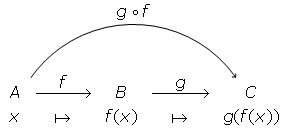
\includegraphics[width=3.0061in]{img/set7.jpg}
\end{center}
\smallskip\par

\begin{exemple}
Considerem les aplicacions $f:\mathbb{R}\longrightarrow\mathbb{R}$ i $g:%
\mathbb{R}\longrightarrow\mathbb{R}$ definides per $f(x)=x+1$ i $g(x)=1-2x$.
Volem calcular l'aplicació composta de $f$ amb $g$.
\end{exemple}

\begin{solucio}
Segons la definició, tenim%
\begin{align*}
(g\circ f)(x) & =g\left( f(x)\right) \\
& =g(x+1) \\
& =1-2(x+1) \\
& =1-2x-2 \\
& =-1-2x
\end{align*}
\end{solucio}

\begin{observacio}
Volem fer dues observacions importants:

\begin{itemize}
\item És important assenyalar que la composició $g\circ f$ de dues
aplicacions $f$ i $g$ està definida, tal com l'hem introduïda, quan el conjunt d'arribada de $f$
coincideix amb el conjunt de sortida de $g$. Més generalment, n'hi ha prou que la imatge de $f$
estigui continguda en el domini de $g$.

\item Observa que en l'expressió $g\circ f$ les aplicacions apareixen
escrites en ordre invers al d'actuació, que és: primer $f$ i després $g$.
\end{itemize}
\end{observacio}

\subsection{Aplicació inversa}

Donada una aplicació $f:A\longrightarrow B$ bijectiva, l'aplicació $%
g:B\longrightarrow A$ definida per
\begin{equation*}
\begin{array}{ccc}
g(y)=x & \Longleftrightarrow & f(x)=y%
\end{array}
\end{equation*}
es diu \textbf{aplicació inversa} de $f$ i és habitual denotar-la
per $f^{-1}$. Segons la definició, és immediat comprovar que%
\begin{equation*}
f^{-1}\circ f=I_{A}\text{ \ \ i \ \ }f\circ f^{-1}=I_{B}
\end{equation*}
on les aplicacions $I_{A}:A\longrightarrow A$ i $I_{B}:B\longrightarrow B$
definides per $I_{A}(x)=x$ per a tot $x\in A$ i $I_{B}(x)=x$ per a tot $x\in
B$ es diuen, respectivament, l'aplicació \textbf{identitat} d'$A$ i
l'aplicació identitat de $B$\textbf{. }

\begin{exemple}
Considerem l'aplicació $f:\mathbb{R}-\left\{ 1\right\} \longrightarrow
\mathbb{R}-\left\{ 2\right\} $ definida per%
\begin{equation*}
f(x)=\frac{2x+1}{x-1}
\end{equation*}
(a) Provarem que $f$ és bijectiva i (b) calcularem l'aplicació
inversa.
\end{exemple}

\begin{solucio}
(a) Si $x,y\in\mathbb{R}-\left\{ 1\right\} $ i suposem que $f(x)=f(y)$,
llavors
\begin{align*}
\frac{2x+1}{x-1} & =\frac{2y+1}{y-1} \\
2xy-2x+y-1 & =2xy+x-2y-1 \\
3y & =3x \\
y & =x
\end{align*}
i, per tant, $f$ és injectiva. Si $y\in\mathbb{R}-\left\{ 2\right\} $ i
fem $f(x)=y$, llavors%
\begin{align*}
\frac{2x+1}{x-1} & =y \\
2x+1 & =xy-y \\
1+y & =xy-2x \\
1+y & =x(y-2) \\
\frac{1+y}{y-2} & =x
\end{align*}
Per tant, donat $y\in\mathbb{R}-\left\{ 2\right\} $, existeix
\begin{equation*}
\frac{1+y}{y-2}\in\mathbb{R}-\left\{ 1\right\}
\end{equation*}
i es compleix%
\begin{equation*}
f\left( \frac{1+y}{y-2}\right) =y\text{.}
\end{equation*}
Això vol dir que $f$ també és exhaustiva i, en conseqüència, $f$ és bijectiva.

(b) Com que per a tot $x\in\mathbb{R}-\left\{ 1\right\} $ i $y\in \mathbb{R}%
-\left\{ 2\right\} $, es compleix
\begin{equation*}
\begin{array}{ccc}
\frac{1+y}{y-2}=x & \Longleftrightarrow & \frac{2x+1}{x-1}=y%
\end{array}
\end{equation*}
llavors%
\begin{equation*}
f^{-1}(y)=\frac{1+y}{y-2}
\end{equation*}
Substituint ara $y$ per $x$, obtenim%
\begin{equation*}
f^{-1}(x)=\frac{1+x}{x-2}\text{.}
\end{equation*}
\end{solucio}

\subsection{Cardinal d'un conjunt}

En aquest apartat precisarem la noció intuïtiva que tots tenim de
nombre d'elements d'un conjunt finit.

\bigskip

Diem que dos conjunts $A$ i $B$ són \textbf{equipotents} quan existeix
una aplicació bijectiva d'$A$ en $B$. Ara podem associar a cada conjunt $%
A$ el que es diu \textbf{cardinal} o \textbf{potència} d'$A$ que es
denota per $\#A$. El cardinal d'un conjunt es defineix de manera que es
compleixi la següent condició: Dos conjunts tenen el mateix cardinal
si i només si són equipotents.

\bigskip

Si $U$ és l'univers i considerem en $\mathcal{P}(U)$ la relació de
equipotència $\sim$ definida per%
\begin{equation*}
\begin{array}{ccc}
A\sim B & \Longleftrightarrow & \#A=\#B\text{,}%
\end{array}
\end{equation*}
és immediat comprovar que $\sim$ és una relació d'equivalència en $\mathcal{P}(U)$ i cada classe es diu un \textbf{nombre cardinal}.
En altres paraules, $n$ és un nombre cardinal si existeix un conjunt $A$
tal que $\#A=n$.

\bigskip

Així, tots els conjunts equipotents a un conjunt unitari com, per
exemple , $\left\{ \emptyset\right\} $, direm que tenen cardinal $1$, tots
els conjunts equipotents a un parell com, per exemple, $\left\{ \emptyset
,\left\{ \emptyset\right\} \right\} $ tenen cardinal $2$, i així
successivament. Admetem que el cardinal del conjunt buit és $0$, és
a dir, $\#\emptyset=0$.

\bigskip

Intuïtivament, és clar que un conjunt finit no pot ser equipotent a
un dels seus subconjunts propis. Tanmateix, això és possible per a
conjunts infinits. Per exemple, el conjunt dels nombres naturals $\mathbb{N}$
és equipotent amb el següent subconjunt propi format pels parells:
\begin{equation*}
P=\left\{ 2n:n\in\mathbb{N}\right\}
\end{equation*}
ja que l'aplicació%
\begin{equation*}
\begin{array}{ccc}
\mathbb{N} & \longrightarrow & P \\
n & \longmapsto & 2n%
\end{array}
\end{equation*}
és bijectiva. Aquest fet justifica la següent definició.

\bigskip

Diem que un conjunt $A$ és \textbf{infinit} si $A$ és equipotent amb
un subconjunt propi de $A$. Si un conjunt no és infinit, llavors diem
que és \textbf{finit}. D'aquesta manera, per a dos conjunts finits $A$ i
$B$, evidentment tenim que $A$ és equipotent a $B$ si i només si $A$
i $B$ contenen el mateix nombre d'elements. Per als conjunts infinits, la
idea "tenir el mateix nombre d'elements" és vaga, mentre que la idea que
$A$ sigui bijectable amb $B$ conserva la seva claredat.

\bigskip

Finalment, diem que un conjunt $A$ és \textbf{infinit numerable} si $A$
és equipotent al conjunt dels nombres naturals $\mathbb{N}$, i diem
simplement \textbf{numerable} si $A$ és finit o infinit numerable.

\subsubsection{Propietats per a conjunts finits}

Les fórmules més usuals (encara que no les úniques) que
relacionen els cardinals i les operacions entre conjunts són:

\begin{enumerate}
\item $\#\left( A\cup B\right) =$ $\#A+$ $\#B-$ $\#\left( A\cap B\right) $

\item $\#\left( A\cup B\cup C\right) =$ $\#A+$ $\#B+$ $\#C-$ $\#\left( A\cap
B\right) -$ $\#\left( A\cap C\right) -$ $\#\left( B\cap C\right) +$ $%
\#\left( A\cap B\cap C\right) $

\item $\#\complement A=$ $\#U-\#A$

\item $\#\left( A\times B\right) =\#A\cdot\#B$

\item $\#\mathcal{P}(A)=2^{\#A}$
\end{enumerate}

Les demostracions d'aquestes propietats les trobaràs en els exercicis
resolts.

\begin{exemple}
En un examen de Matemàtiques i Física han concorregut 100 alumnes.
Sabent que Física l'han aprovat 60 alumnes, Matemàtiques 48 i que
el nombre d'alumnes que han aprovat totes dues assignatures ha estat 30,
volem esbrinar el nombre d'alumnes que no han aprovat cap assignatura en
aquest examen.
\end{exemple}

\begin{solucio}
Tenim els següents conjunts: el conjunt $U$ d'alumnes que s'examinen, el
conjunt $A$ d'alumnes que han aprovat Física i el conjunt $B$ d'alumnes
que han aprovat Matemàtiques. Per l'enunciat del problema, se sap que $%
\#U=100$, $\#A=60$, $\#B=48$ i $\#(A\cap B)=30$. El conjunt d'alumnes que han
aprovat alguna assignatura és $A\cup B$ i el nombre d'elements d'aquest
conjunt és%
\begin{align*}
\#\left( A\cup B\right) & =\#A+\#B-\#\left( A\cap B\right) \\
& =60+48-30 \\
& =78
\end{align*}
Llavors, el nombre d'alumnes que no han aprovat cap assignatura és $22$
perquè aquest nombre és el cardinal del conjunt $\complement(A\cup B)
$ i es compleix que%
\begin{align*}
\#\complement(A\cup B) & =\#U-\#\left( A\cup B\right) \\
& =100-78 \\
& =22\text{.}
\end{align*}
\end{solucio}
